%
% klassischerHarmonischerOszillator.tex
%
% (c) 2020 Prof Dr Andreas Müller, Hochschule Rapperswil
%
% !TEX root = ../../buch.tex
% !TEX encoding = UTF-8
%

\section{Der klassische harmonische Oszillator\label{fourier:section:derKlassischeHarmonischeOszillator}}
\kopfrechts{Der klassische harmonische Oszillator}%

In diesem Abschnitt wird die Energie eines ungedämpften Federpendels näher untersucht.
Ein ungedämpftes Federpendel ist ein typisches Beispiel für einen harmonischen Oszillator.
Die Abbildung~\ref{fourier:fig:federpendel} zeigt anschaulich, wie sich das Pendel um seine Ruhelage bewegt und wie sich dabei die potentielle Energie verändert.
\index{potentielle Energie}%
%
% fig-federpendel.tex
%
% (c) 2025 Prof Dr Andreas Müller
%
\begin{figure}
\centering
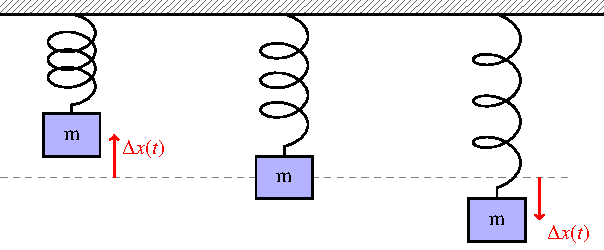
\includegraphics{papers/fourier/images/federpendel.pdf}
\caption{Federpendel
\label{fourier:fig:federpendel}}
\end{figure}
Im folgenden Abschnitt~\ref{fourier:subsection:derQMHarmonischeOszillator} wird der harmonische Oszillator dann im Rahmen der Quantenfeldtheorie betrachtet.
\index{harmonischer Oszillator}%

Die Gesamtenergie \( E \) eines mechanischen Systems ergibt sich als Summe der kinetischen Energie \( E_{\text{kin}} \) und der potentiellen Energie \( E_{\text{pot}} \):  
\begin{equation}  
	E = E_{\text{kin}} + E_{\text{pot}}.  
\end{equation}
Eine ungedämpfte Schwingung ist dadurch gekennzeichnet, dass keine Energieverluste durch Reibung oder andere hemmende Einflüsse auftreten.  
Die Energie des Systems bleibt daher konstant.  
Unter der Annahme, dass die rücktreibende Kraft linear von der Auslenkung abhängt, ergibt sich daraus das Modell des harmonischen Oszillators.
\index{rücktreibende Kraft}%

Die kinetische und die potentielle Energie lassen sich wie folgt ausdrücken:  
\begin{align}  
	E_{\text{kin}} &= \frac{1}{2} m v^2, \\  
	E_{\text{pot}} &= \frac{1}{2} k x^2,  
\end{align}  
wobei \( m \) die Masse des Körpers, \( v \) seine Geschwindigkeit, \( k \) die Federkonstante und \( x \) die Auslenkung aus der Ruhelage ist.
\index{Federkonstante}%
Daraus ergibt sich für die Gesamtenergie:  
\begin{equation}  
	E = \frac{1}{2} m v^2 + \frac{1}{2} k x^2.  
\end{equation}

Um die Energie in Abhängigkeit von Impuls und Ort auszudrücken, wird der klassische Impuls \( p = m v \) verwendet.  
Durch Umstellen erhält man:  
\[
	v = \frac{p}{m}.  
\]  
Setzt man dies in die Gleichung für \( E \) ein, ergibt sich:  
\begin{equation}\label{fourier:equation:derKlassischeHarmonischeOszillator}  
	E = \frac{1}{2} m {\left(\frac{p}{m}\right)}^{2} + \frac{1}{2} k x^{2} = \frac{p^{2}}{2m} + \frac{1}{2} k x^{2}.
\end{equation}

%
% fig-federpendel.tex
%
% (c) 2025 Prof Dr Andreas Müller
%
\begin{figure}
\centering
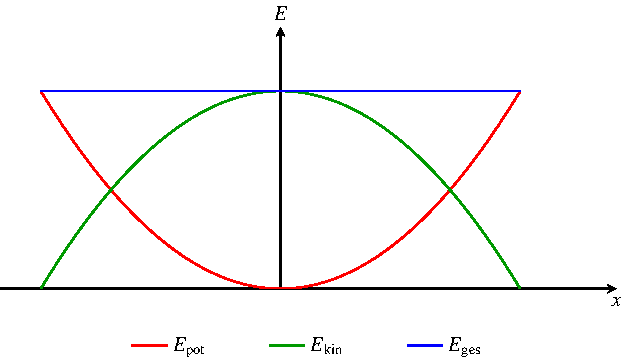
\includegraphics{papers/fourier/images/hmo_energiediagramm.pdf}
\caption{Darstellung der Gesamtenergie eines harmonischen Oszillators in Abhängigkeit von Ort und Impuls, aufgeteilt in kinetische und potentielle Energie.%
\label{fourier:fig:hmo_energiediagramm}}
\end{figure}

Zur Veranschaulichung dient Abbildung~\ref{fourier:fig:hmo_energiediagramm}.
Damit ist die Energie des klassischen harmonischen Oszillators in Abhängigkeit von Impuls \( p \) und Ort \( x \) dargestellt.  
Diese Darstellung der Gesamtenergie in Abhängigkeit von Impuls \( p \) und Ort \( x \) ist besonders wichtig,  
da sie die Grundlage für die spätere Formulierung des Hamilton-Operators in der Quantenmechanik bildet.
